\documentclass[8pt,a4paper,landscape]{extarticle}
% -- Layout ----
\usepackage[top=0.6cm, bottom=0.6cm, left=0.5cm, right=0.5cm, landscape]{geometry}

% -- Titles ----
\usepackage[
  tiny,                     % text size title
  compact                   % reduce vertical space before/after title
]{titlesec}
% \titlespacing*
\titleformat{\section}{\normalfont\small\bfseries}{\thesection}{0em}{} % Remove space before and after section titles
\titleformat{\subsection}{\normalfont\small\bfseries}{\thesubsection}{0em}{} % Remove space before and after subsection titles
\titlespacing*{\section}{0pt}{0pt}{0pt} % Remove space before/after section titles
\titlespacing*{\subsection}{0pt}{0pt}{0pt} % Remove space before/after subsec titles

% -- Colors ----
\usepackage[dvipsnames]{xcolor}
\definecolor{dmm}{RGB}{192,192,192} % Define a custom dimmed text color
\definecolor{cmt}{RGB}{61,123,123}

% -- Math ------
\usepackage{mathtools}
\usepackage{amssymb}
\usepackage{turnstile}%better vdash

% -- Lists -----
\usepackage[inline]{enumitem}
\setlist{noitemsep}% Remove vspace between items
% Set vspace before and after  list environments as well as the left margin
\setlist[itemize,1]{leftmargin=.6em,labelindent=0pt,labelsep=2pt,
  topsep=1pt,partopsep=1pt}
\setlist[enumerate,1]{leftmargin=1em,labelindent=0pt,labelsep=2pt,
  topsep=1pt,partopsep=1pt}
\setlist[itemize,2]{leftmargin=.3em,labelindent=1pt,topsep=1pt,partopsep=1pt}
\setlist[enumerate,2]{leftmargin=0.2em,labelindent=1pt,topsep=1pt,partopsep=1pt}
\setlist[description]{labelwidth=\linewidth,font=\small\bfseries,leftmargin=1em,topsep=1pt,partopsep=1pt}
% -- Code listing ---
\usepackage{listings}
\lstset{
  aboveskip=3pt,
  belowskip=3pt,
  basicstyle=\small\ttfamily,
  breaklines=true,
  % commentstyle=\upshape\ttfamily,
  captionpos=b,
  commentstyle=\color{cmt},
  frame=single,
  keepspaces=false,
  keywordstyle=\bfseries,
  showspaces=false,
  showstringspaces=false,
  showtabs=false,
  tabsize=2,
}

% Parse Trees
\usepackage{tikz}
\usetikzlibrary{ arrows, automata, bbox, calc, positioning,  decorations.pathmorphing, decorations.pathreplacing, decorations.shapes, }
\tikzset{
% ->, % makes the edges directed
>=stealth', % makes the arrow heads bold
node distance=1cm, % specifies minimum distance between two nodes
% small/.style={},
every state/.style={thick}, % sets the properties for each ’state’ node
every node/.style={inner sep=1pt},
initial text=start, % sets the text that appears on the start arrow
}

% Place a figure env right here via [H] option
\usepackage{float}

% Side by side figure
\usepackage{subcaption}
% \usepackage{caption}
% \captionsetup{belowskip=0pt, aboveskip=0pt}


% -- Multi-Col layout --
\usepackage{multicol}

% No indentation
\setlength\parindent{0pt}
\setlength\abovedisplayskip{-5pt}
\setlength\belowdisplayskip{-5pt}
\setlength\abovedisplayshortskip{-4pt}
\setlength\belowdisplayshortskip{-4pt}
\newcommand{\gor}{\;|\;}
\newcommand{\num}{\texttt{\#}~}
\renewcommand{\arraystretch}{1.2}


\begin{document}
% Suppress page number for all pages
\pagestyle{empty}

% Notes begin
\begin{multicols*}{3}
\section*{Jargon}
\begin{description}

\item[synchronous iteration] several procs start together at the beginning of each iteration and the next iteration must wait for all procs to finish current iteration

\item[SPMD] all procs execute the same program (Single Program, SP) in parallel (except for a small number of procs such as root), but each has its own set of data (Multiple Data). In src code, usually a proc ID is used to uniquely label a proc

\item[Motivation for parallelism]
  \begin{enumerate*}
  \item speed/performance (1h vs 1w)
  \item tackle larger-scale problems
  \item keep power consumption and heat dissipation under control
  \item more $\cdots$
  \end{enumerate*}

\item[peak flops/sec] $ = \# \text{cores} \times [\# \text{sockets}] \times \# \text{flops} \times \text{freq}$

\item[speedup (hard due to overheads)]
  \begin{enumerate*}
  \item idling (unbalanced load, sync, serial parts, etc)
  \item splitting computation into tasks
  \item communications among processes
  \end{enumerate*}

\item[speedup (fixed problem size) and efficiency] $S_p = \frac{T_{seq}}{T_{par}} (\geq 1)\qquad E_p = \frac{S_{p}}{p} (0 < E_p \leq 1)$

% \item[efficiency] $E_p = \frac{S_{p}}{p} (0 < E_p \leq 1)$

\item[embarrassingly (easy) parallel] aka. perfectly parallel, delightfully parallel or pleasingly parallel, where problem can be easily divided into independent parts and solved without communication

\item[strong scalability] fixed problem size + increasing $\# p \rightarrow$ perf $\downarrow$

\item[weak scalability] increasing $\# p$ and problem size $\rightarrow$ perf $\downarrow$

\item[communication latency] time taken to communicate a msg between 2 procs in a network

\item[minimal routing] takes 1 of shortest paths (XY-routing; E-cube)

\item[non-minimal routing] route the message along a longer path to avoid network congestion

\item[deterministic] routing determines a unique path \emph{solely} based on src and dest nodes

\item[adaptive] routing uses info on network state to determine message path

\item[walltime] the actual time taken from the start of a computer program to the end. aka. elapsed real time, real time, wall-clock time
\item[flops] floating-point operations (add, subtract, multiply, divide) per second
\item[ceil] ceil(n,p) = $(n + p - 1) / p$ especially when $n$ isn't evenly divisible by $p$

\item[synchronous] 2 procs A, B. A will only start sending when B explicitly signals it is ready to receive.  If not, A just waits (also blocks).  In such mode, two procs communicate with each other directly.

\item[asynchronous] All concurrent tasks execute asynchronously; possible to implement any parallel algorithm.  However, it is hard to reason about the program because of non-deterministic behavior due to race conditions.

\item[loosely synchronous] a good compromise between aysnc and sync.  Tasks and subtasks synchronize to perform interactions (easy to debug), while between interactions, tasks execute completely asynchronously.

\item[blocking, non-buffered] A sends and B recvs, no system buffer available.  A must hold the data (A being idle and blocking) until B is ready to receive.

\item[blocking, buffered] data/message can be copied into a system-controlled block of memory (buffer on A or B or both) so A can continue to execute.  When B is ready, it copies the buffered data into its own appropriate memory.  A \textbf{common} implementation is to buffer relatively small messages and switch to non-buffered mode for large messages (blocking too).  In general, better to write programs with bounded buffer requirements.  This blocking time is only the period of copying data into/from buffer.
\item[non-blocking] generally accompanied by a \texttt{check-status} operation.  Upon return from non-blocking send/recv, the proc is free to perform any computation that doesn't require communication.  Later the proc \textbf{checks} if non-blocking op has completed and wait for its completion if needed.
\item[communication domain] a set of processes allowed to communicate with each other.  Info about this domain is stored in vars of type \texttt{MPI\_Comm} aka \textbf{communicators} (used as arg to all message transfer MPI routines and they uniquely identify procs). One proc can belong to many different (possibly overlapping) communication domains.  \texttt{MPI\_COMM\_WORLD} includes all procs in parallel execution as they all may need to talk to each other.

\item[one-to-all broadcast] a single process sends \textbf{identical} data to all other processes or to a subset of them.  Initially, only the source process has the data of size $m$ that needs to be broadcast.  At the termination of the procedure, there are $p$ copies of the initial data --- one belonging to each process.

\item[all-to-one reduction] each of the p participating processes starts with a buffer $M$ containing $m$ words.  The data from all processes are combined through an associative operator and accumulated at a single destination process into one buffer of size $m$.  Reduction can be used to find the sum, product, maximum, or minimum of sets of numbers

\item[latency] At the logical level, a memory system (of multiple levels of caches) takes in a request for a memory word and returns a block of data of size $b$ containing the requested word after $l$ nanoseconds, referred to as the \textbf{latency} of the memory.  As an analogy, if water comes out of the end of a fire hose 2 seconds after a hydrant is turned on, then the latency of the system is 2 seconds.


\item[bandwidth] The rate at which data can be pumped from the memory to the processor determines the bandwidth of the memory system.  How much data (per unit time) gets transferred from memory to processor.


\item[hit ration] The fraction of data references satisfied by the cache is called the cache hit ratio of the computation on the system.   The effective computation rate of many applications is bounded \emph{not} by the processing rate of the CPU, but by the rate at which data can be pumped into the CPU.  Such computations are referred to as being \textbf{memory bound}.


\item[temporal locality] If at one point a particular mem location is ref-ed, then it's likely that the same location will be ref-ed again soon

\item[spatial locality] Data that is accessed or referenced spatially close to each other (\texttt{a[i-1],a[i],a[i+1]}) is likely to be accessed again in the near future

\item[recursive decomposition] a method for inducing concurrency in problems that can be solved using the divide-and-conquer strategy.  A problem is solved by first dividing it into a set of independent subproblems. Each subproblem is solved by recursively applying a similar division into smaller subproblems followed by a combination of their results. (quicksort)


\item[data decomposition] a powerful/commonly used method for deriving concurrency in algorithms that operate on large data structures.  The decomposition of computations is done in two steps.  First, the data on which the computations are performed is partitioned; second, this data partitioning is used to induce a partitioning of the computations into tasks. The operations these tasks perform on different data partitions are usually similar or are chosen from a small set of operations (LU factorization).


\item[partitioning output data] In many computations, each element of the output can be computed naturally independently of others as a function of the input. In such computations, a partitioning of the output data automatically induces a decomposition of the problems into tasks, where each task is assigned the work of computing a portion of the output. (matrix-multiplication)


\item[partioning input data] When impossible to split output data, it is possible to partition the input data, and then use this partitioning to induce concurrency. A task is created for each partition of the input data and this task performs as much computation as possible using these local data. Note that the solutions to tasks induced by input partitions may not directly solve the original problem. In such cases, a follow-up computation is needed to combine the results. (sum of n elements)

\item[exploratory decomposition] is used to decompose problems whose underlying computations correspond to a search of a space for solutions. In exploratory decomposition, we partition the search space into smaller parts, and search each one of these parts concurrently, until the desired solutions are found. For an example of exploratory decomposition, consider the 15-puzzle problem.


\item[speculative decomposition] used when a program may take one of many possible computationally significant branches depending on the output of other computations that precede it. In this situation, while one task is performing the computation whose output is used in deciding the next computation, other tasks can concurrently start the computations of the next stage. The speedup due to speculative decomposition can add up if there are multiple speculative stages. (discrete event simulation)


\item[stream parallelism] simultaneous execution of different programs on a data stream


\item[startup time $t_s$] The startup time is the time required to handle a message at the sending and receiving nodes: the time to prepare the message (adding header, trailer, and error correction information), the time to execute the routing algorithm, and the time to establish an interface between the local node and the router. This delay is incurred only once for a single message transfer

\item[per-hop time $t_h$ (aka. node latency)] After a message leaves a node, it takes a finite amount of time to reach the next node in its path. The time taken by the header of a message to travel between two directly-connected nodes in the network is called the per-hop time.


\item[per-word transfer time $t_w$] If the channel bandwidth is $r$ words/s, then each word takes time $tw = 1/r$ to traverse the link. This time is called the per-word transfer time. This time includes network as well as buffering overheads.




\end{description}

\section*{Amdahl's law (strong scaling law, \textbf{L5P5})}
\begin{equation}
  \label{eq:amdahl}
  S_p = \frac{T_{seq}}{T_{par}} = \frac{p}{pf + (1-f)} = \frac{1}{f + \frac{1-f}{p}}
\end{equation}
where $f$ is the serial portion that cannot be parallelized
\begin{tabular}{c|c}
  \hline
  \multicolumn{2}{l}{$S \rightarrow ? $ if run on 1000 CPU and 10\% ($f$) remains sequential} \\
  \hline
  $S_{ser} \quad p = 1$ & $S_{par} \quad p = 1000$  \\
  \hline
  2GFLOP/s  & $S_{ser} \times \frac{1}{0.1 + \frac{1-0.1}{1000}} \approx 9.91 \times S_{ser} = 19.82$ GFLOP/s \\
  \hline
\end{tabular}
\begin{tabular}{l|r}
  \hline
  \multicolumn{2}{l}{Calc $Ax=b$ where $A$ is $M \times N$ matrix} \\
  \multicolumn{2}{l}{$T_{ser} = 2MNT$ where $T$ is time for single float op} \\
  \multicolumn{2}{l}{$T_{sort} = 2M\log_2(M)T$ where sorting can only be sequential} \\
  \hline
  $T_{ser} \quad p = 1$ & $T_{par} \quad p = P \rightarrow \infty$ \\
  \hline
  $2MNT + 2M\log_2(M)T$ & $\frac{2MNT}{P} + 2M\log_2(M)T$ \\
  \hline
\end{tabular}
\begin{align*}
  S & = \frac{T_{ser}}{T_{par}} = \frac{2MNT + 2M\log_2(M)T}{\frac{2MNT}{P} + 2M\log_2(M)T} \\
    & = \frac{2MNT + 2M\log_2(M)T}{2M\log_2(M)T} \quad (P \rightarrow \infty \therefore \frac{2MNT}{P} \rightarrow 0) \\
    & = \frac{N}{\log_2(M)} + 1
\end{align*}
\section*{Gustafson's law (weak scaling law, \textbf{L5P7})}
\(S_p = p - f(p-1)\) where $f$ is the serial portion (independent of $p$ and problem size) and has the following assumptions:
\begin{enumerate}
\item the serial portion is kept constant when scaling problem size ($N$)
\item the perfectly parallelizable portion scales linearly with $\#p$ if $N$ scales linearly, then $T_{par}$ is kept constant.
\end{enumerate}

\section*{Moore's Law and Dennard Scaling (\textbf{L1P17})}

\begin{itemize}
  \item the two laws (\emph{underpin} exponential perf. increase of microprocessors)
  \item \textbf{Moore's} law (transistors doubles $\ne$ perf. doubles, \textbf{L1P17})
  \item \textbf{Dennard} Scaling (\textbf{L1P18-19}, examples below)
  \item[] $P = QfCV^{2}$ ($Q$: \# of transistors, $f$ frequency)
  \begin{tabular}{c|ccc}
    \hline
    \multicolumn{4}{l}{scale down feature size by  $\frac{1}{k}\approx 0.7$, then $k\approx 1.42, k^{2}\approx 2$} \\
    \hline
    & \# of trans. $Q$ & freq. $f$ & power usage $P$  \\
    \hline
    $Q_{0} = Q_{k}$ & unchanged & $f_k = k \cdot f_0$ & $P_k = (\frac{1}{k})P_0$\\
    $P_{0} = P_{k}$ & $Q_k = k^{2} \cdot Q_0$ & $f_k = k \cdot f_0$ & unchanged  \\
    \hline
    \multicolumn{4}{l}{feature size $\geq$ 100nm or $VI_{\text{leakage}}$  dominates power consumption} \\
    \hline
  \end{tabular}
\item these two also \emph{undermine} parallel computing however (\textbf{L1P21})
\item end of Dennard scaling $\rightarrow$ multicore era (\textbf{L1P23-24})
\end{itemize}

\section*{Flynn's Taxonomy (\textbf{L2-3P12-14})}
\begin{tabular}{l|p{4cm}l}
  \hline
  Type & Note & Example \\
  \hline
  SISD & 1 ix process a stream data  & von Neumann model \\
  SIMD & 1 ix stream broadcast to many & vector processor; Quardrics\\
  MISD & no such machines  & - \\
  MIMD & each proc with its own ix/data & Gadi; most of top 500 \\
  \hline
\end{tabular}

\section*{Store-and-Forward (SF) routing (\textbf{L7P5})}
\begin{equation*}
  t_{\text{comm}} = t_{s} + l(t_h + mt_w) \quad m \text{ is message size}; l \text{ is link num}
\end{equation*}
\begin{equation*}
  t_{\text{comm}} \approx t_{s} + lmt_w (\because t_h \ll mt_w \text{even for small} m)
\end{equation*}
\section*{Cut-Through (CT) routing (\textbf{L7P6})}
\begin{equation*}
  t_{\text{comm}} = t_{s} + lt_h + mt_w
\end{equation*}
If the communication is between nearest neighbors (that is, $l = 1$), or if the message size is small, then $T_{\text{comm}}$ is similar for store-and-forward and cut-through routing
\section*{One-to-all SF on different networks (\textbf{L7P9-10})}
\begin{tabular}{c|lc}
  \hline
  Network & Communication Cost & Source \\
  \hline
  Ring & $T_{\text{one-all}} = (t_s + t_{w}m) \frac{p}{2}$  & \textbf{L7P9} \\
  2D Mesh & $T_{\text{one-all}} = 2(t_s + t_{w}m) \frac{\sqrt{p}}{2}$ & \\
  3D Mesh & $T_{\text{one-all}} = 3(t_s + t_{w}m) \frac{\sqrt[3]{p}}{2}$ &  \\
  Hypercude & $T_{\text{one-all}} = (t_s + t_{w}m) \log_2 p$ & \textbf{L7P10} \\
  \hline
  \multicolumn{3}{l}{one-to-all broadcast with SF routing is \textbf{fastest} on hypercube}\\
  \hline
\end{tabular}
\section*{One-to-all CT on different networks (\textbf{L7P11-13})}
\begin{tabular}{c|l|c}
  \hline
  Network & Communication Cost & Source \\
  \hline
  Ring & $T_{\text{one-all}} = \log_2 p(t_s + mt_{w}) + t_h(p-1)$ & \textbf{L7P11} \\
  2D Mesh & $T_{\text{one-all}} = 2\log_2 (\sqrt{p})(t_s + mt_{w}) + 2t_h(\sqrt{p}-1) $ & \textbf{L7P12}\\
  Binary Tree & $T_{\text{one-all}} = \log_2(p)(t_s + mt_{w})+(\sum^{\log_2(p)}_{i=1}2i)t_h$ & \textbf{L7P13} \\
  \hline
  \multicolumn{3}{l}{one-to-all broadcast with CF does \emph{not} improve (not faster than SF)}\\
  \multicolumn{3}{l}{because of exclusively nearest-neighbor communication}\\
  \hline
\end{tabular}

\section*{All-to-All Store-and-Forward (SF) Routing (\textbf{L7P14-16})}
\begin{tabular}{c|l|c}
  \hline
  Network & Communication Cost & Source \\
  \hline
  Ring & $T_{\text{all-all}} = (p-1)(t_s + t_h mt_{w})$ & \textbf{L7P14} \\
  2D Torus & $T_{\text{all-all}} = 2(t_s + t_h)(\sqrt{p} - 1)+mt_{w}(p-1)$ & \textbf{L7P15}\\
  Hypercube & $T_{\text{all-all}} = 2\log_2(p)(t_s + t_h)+2(p-1)mt_w$ & \textbf{L7P16} \\
  \hline
\end{tabular}

\section*{Methods for containing interaction overheads}
\begin{enumerate}
\item Maximizing Data Locality
  \begin{itemize}
  \item Minimize Volume of Data-Exchange (minimize the overall volume of shared data, akin to maximizing the temporal data locality)
  \item Minimize Frequency of Interaction (there is a relatively high startup cost associated with each interaction on many architectures)
  \end{itemize}
\item Minimizing Contention and Hot Spots
\item Overlapping Computations with Interactions (init interaction early enough so that it's completed before it's needed for computation)
\item Replicating Data or Computations
\item Using Optimized Collective Interaction Operations
\item Overlapping Interactions with Other Interactions
\end{enumerate}
\section*{Parallel Algorithm Models}
\begin{itemize}
\item Data-Parallel (data parallelism, GPU) tasks are statically or semi-statically mapped onto processes and each task performs similar operations on different data
\item Task Graph: interrelationships among the tasks are utilized to promote locality or to reduce interaction costs; typically employed to solve problems in which the amount of data associated with the tasks is large relative to the amount of computation associated with them.
\item Work Pool: a dynamic mapping of tasks onto processes for load balancing in which any task may potentially be performed by any process; no desired premapping of tasks onto processes
\item Master-Slave (manager-worker): one or more master processes generate work and allocate it to worker processes
\item Pipeline or Producer-Consumer: a stream of data is passed on through a succession of processes, each of which perform some task on it
\end{itemize}


% \section*{Matrices Multiplication (Square n $\times$ n)}
\begin{equation*}
  A_{n,n} \times B_{n,n} =
 \begin{bmatrix}
  a_{11} & a_{12} & \cdots & a_{1n} \\
  a_{21} & a_{22} & \cdots & a_{2n} \\
  \vdots  & \vdots  & \ddots & \vdots  \\
  a_{n1} & a_{n2} & \cdots & a_{nn}
 \end{bmatrix}
  \begin{bmatrix}
  b_{11} & b_{12} & \cdots & b_{1n} \\
  b_{21} & b_{22} & \cdots & b_{2n} \\
  \vdots  & \vdots  & \ddots & \vdots  \\
  b_{n1} & b_{n2} & \cdots & b_{nn}
 \end{bmatrix}
\end{equation*}
\begin{align*}
  \label{eq:mmitem}
  C_{ij} & =  \begin{bmatrix}
                a_{i1} \\
                a_{i2} \\
                \vdots \\
                a_{in}
              \end{bmatrix}
              \begin{bmatrix}
                b_{1j} & b_{2j} & \cdots & b_{nj}
              \end{bmatrix} =
           \begin{bmatrix}
                a_{i1} \\
                a_{i2} \\
                \vdots \\
                a_{in}
           \end{bmatrix}
           \cdot
           \begin{bmatrix}
                b_{1j} \\
                b_{2j} \\
                \vdots \\
                b_{nj}
           \end{bmatrix} \\
         & = a_{i1}\cdot b_{1j}+a_{i2}\cdot b_{2j}+\cdots+a_{in}\cdot b_{nj} \\
         & = \sum_{i,j=1}^{n}a_{ij}\cdot b_{ji}
\end{align*}

\lstinputlisting[language=C,linerange={4-17}]{sec/matrixmul1.c}

\section*{Mapping 2D array to 1D array in \texttt{C}}
\begin{itemize}
\item given a grid of size $M$ by $N$ where $M$ is row $\#$ and $N$ is column $\#$
\item halo layer around only 4 edges: top, bottom, left, right
\item corner elements of halo: (0,0), (0,$N+1$), ($M+1$,$N+1$), ($M+1$,0)
\item corner elements of interior field: (1,1), (1,$N$), ($M,N$), ($M$,1)
\item using 1D array \texttt{u[]} to store all points, thus \texttt{u} size $(M+2)\times(N+2)$
\item parallel algorithm implementation on $P$ by $Q$ process grid
\item use a 2-stage halo exchange: top-bottom then left-right
\end{itemize}
% M by N matrix
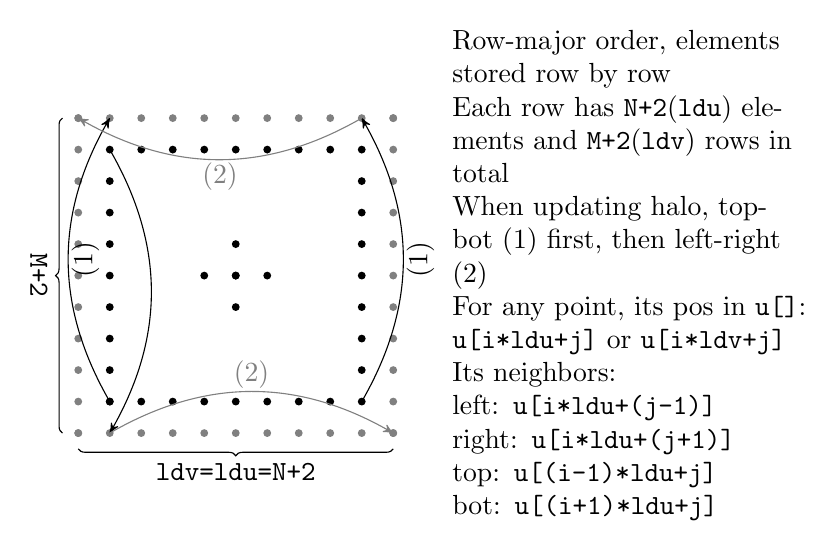
\begin{tikzpicture}
  [halo/.style={circle,fill,gray,inner sep=1pt},
  innr/.style={circle,fill,inner sep=1pt},
  info/.style={inner sep=1ex,font=\small}]

  % halo
  \foreach \i in {0,0.4,...,4} {
    \node at (\i,0)[halo]{}; %halo top
    \node at (\i,4)[halo]{}; %halo bot
    \node at (0,\i)[halo]{}; %halo left
    \node at (4,\i)[halo]{}; %halo right
  }

  % halo
  \foreach \j in {0.4,0.8,...,3.6} {
    \node at (\j,3.6)[innr]{}; %inner top
    \node at (\j,0.4)[innr]{}; %inner bot
    \node at (0.4,\j)[innr]{}; %inner left
    \node at (3.6,\j)[innr]{}; %inner right
  }
  \node at (3.6,3.6)[innr]{};

  \foreach \m in {1.6,2.0,2.4} {
    \node at (\m, 2.0)[innr]{};
    \node at (2.0, \m)[innr]{};
  }

  % neighbors

  \draw[decorate,decoration={brace,mirror}] (-.2,4.0) -- (-.2,0); %left
  \draw[decorate,decoration={brace,mirror}] (0,-.2) -- (4.0,-.2); %bot
  \node at (-.5,2)[rotate=-90]{\texttt{M+2}};
  \node at (2,-.5)[](ldu){\texttt{ldv=ldu=N+2}};

  % halo src to dest
  \path[->] (0.4,0.4) edge[bend left] node[below,sloped]{(1)} (0.4,4); %top halo left
  \path[->] (3.6,0.4) edge[bend right] node[below,sloped]{(1)} (3.6,4);%top halo right
  \path[->] (0.4,3.6) edge[bend left] (0.4,0);

  \path[->] (3.6,4) edge[bend left,gray] node[below,sloped]{(2)} (0,4);
  \path[->] (0.4,0) edge[bend left,gray] node[above,sloped]{(2)} (4,0);

  % txt
  \node[xshift=7cm,yshift=2cm,text width=4.5cm]
  {
    Row-major order, elements stored row by row\\
    Each row has \texttt{N+2}(\texttt{ldu}) elements and \texttt{M+2}(\texttt{ldv}) rows in total\\
    When updating halo, top-bot (1) first, then left-right (2) \\
    For any point, its pos in \texttt{u[]}:
    \texttt{u[i*ldu+j]} or \texttt{u[i*ldv+j]}\\
    Its neighbors:\\
    left:  \texttt{u[i*ldu+(j-1)]} \\
    right: \texttt{u[i*ldu+(j+1)]}\\
    top:   \texttt{u[(i-1)*ldu+j]}\\
    bot:   \texttt{u[(i+1)*ldu+j]}
  };
\end{tikzpicture}
      % top left halo, \texttt{u[1] = u[(M+1)*ldu+1]}\\
      % top right halo, \texttt{u[1] = u[(M+1)*ldu+1]}\\
      % bot left halo, \texttt{u[1] = u[(M+1)*ldu+1]}\\
      % bot right halo, \texttt{u[1] = u[(M+1)*ldu+1]}\\
      % left halo, \texttt{u[1] = u[(M+1)*ldu+1]}\\
      % right halo, \texttt{u[1] = u[(M+1)*ldu+1]}\\

\section*{Overhead and resolution of timer}
\begin{itemize}
\item Overhead = $\text{Avg}(\text{overhead}_1,\text{overhead}_2,\cdots,\text{overhead}_n)$
\item Resolution = Smallest diff between any 2 watched times
\end{itemize}
\end{multicols*}
\end{document}
